\documentclass[conference]{IEEEtran}
\IEEEoverridecommandlockouts

% *** CITATION PACKAGES ***
%
\usepackage{cite}
% cite.sty was written by Donald Arseneau
% V1.6 and later of IEEEtran pre-defines the format of the cite.sty package
% \cite{} output to follow that of IEEE. Loading the cite package will
% result in citation numbers being automatically sorted and properly
% "compressed/ranged". e.g., [1], [9], [2], [7], [5], [6] without using
% cite.sty will become [1], [2], [5]--[7], [9] using cite.sty. cite.sty's
% \cite will automatically add leading space, if needed. Use cite.sty's
% noadjust option (cite.sty V3.8 and later) if you want to turn this off.
% cite.sty is already installed on most LaTeX systems. Be sure and use
% version 4.0 (2003-05-27) and later if using hyperref.sty. cite.sty does
% not currently provide for hyperlinked citations.
% The latest version can be obtained at:
% http://www.ctan.org/tex-archive/macros/latex/contrib/cite/
% The documentation is contained in the cite.sty file itself.

% *** GRAPHICS RELATED PACKAGES ***
%
\ifCLASSINFOpdf
  \usepackage[pdftex]{graphicx}
  % declare the path(s) where your graphic files are
  % \graphicspath{{../pdf/}{../jpeg/}}
  \graphicspath{{images/}}
  % and their extensions so you won't have to specify these with
  % every instance of \includegraphics
  \DeclareGraphicsExtensions{.jpeg,.png}
\else
  % or other class option (dvipsone, dvipdf, if not using dvips). graphicx
  % will default to the driver specified in the system graphics.cfg if no
  % driver is specified.
  % \usepackage[dvips]{graphicx}
  % declare the path(s) where your graphic files are
  % \graphicspath{{../eps/}}
  % and their extensions so you won't have to specify these with
  % every instance of \includegraphics
  % \DeclareGraphicsExtensions{.eps}
\fi
% graphicx was written by David Carlisle and Sebastian Rahtz. It is
% required if you want graphics, photos, etc. graphicx.sty is already
% installed on most LaTeX systems. The latest version and documentation can
% be obtained at: 
% http://www.ctan.org/tex-archive/macros/latex/required/graphics/
% Another good source of documentation is "Using Imported Graphics in
% LaTeX2e" by Keith Reckdahl which can be found as epslatex.ps or
% epslatex.pdf at: http://www.ctan.org/tex-archive/info/
%
% latex, and pdflatex in dvi mode, support graphics in encapsulated
% postscript (.eps) format. pdflatex in pdf mode supports graphics
% in .pdf, .jpeg, .png and .mps (metapost) formats. Users should ensure
% that all non-photo figures use a vector format (.eps, .pdf, .mps) and
% not a bitmapped formats (.jpeg, .png). IEEE frowns on bitmapped formats
% which can result in "jaggedy"/blurry rendering of lines and letters as
% well as large increases in file sizes.
%
% You can find documentation about the pdfTeX application at:
% http://www.tug.org/applications/pdftex

% *** MATH PACKAGES ***
%
%\usepackage[cmex10]{amsmath}
% A popular package from the American Mathematical Society that provides
% many useful and powerful commands for dealing with mathematics. If using
% it, be sure to load this package with the cmex10 option to ensure that
% only type 1 fonts will utilized at all point sizes. Without this option,
% it is possible that some math symbols, particularly those within
% footnotes, will be rendered in bitmap form which will result in a
% document that can not be IEEE Xplore compliant!
%
% Also, note that the amsmath package sets \interdisplaylinepenalty to 10000
% thus preventing page breaks from occurring within multiline equations. Use:
%\interdisplaylinepenalty=2500
% after loading amsmath to restore such page breaks as IEEEtran.cls normally
% does. amsmath.sty is already installed on most LaTeX systems. The latest
% version and documentation can be obtained at:
% http://www.ctan.org/tex-archive/macros/latex/required/amslatex/math/

% *** SPECIALIZED LIST PACKAGES ***
%
%\usepackage{algorithmic}
% algorithmic.sty was written by Peter Williams and Rogerio Brito.
% This package provides an algorithmic environment fo describing algorithms.
% You can use the algorithmic environment in-text or within a figure
% environment to provide for a floating algorithm. Do NOT use the algorithm
% floating environment provided by algorithm.sty (by the same authors) or
% algorithm2e.sty (by Christophe Fiorio) as IEEE does not use dedicated
% algorithm float types and packages that provide these will not provide
% correct IEEE style captions. The latest version and documentation of
% algorithmic.sty can be obtained at:
% http://www.ctan.org/tex-archive/macros/latex/contrib/algorithms/
% There is also a support site at:
% http://algorithms.berlios.de/index.html
% Also of interest may be the (relatively newer and more customizable)
% algorithmicx.sty package by Szasz Janos:
% http://www.ctan.org/tex-archive/macros/latex/contrib/algorithmicx/


% *** ALIGNMENT PACKAGES ***
%
%\usepackage{array}
% Frank Mittelbach's and David Carlisle's array.sty patches and improves
% the standard LaTeX2e array and tabular environments to provide better
% appearance and additional user controls. As the default LaTeX2e table
% generation code is lacking to the point of almost being broken with
% respect to the quality of the end results, all users are strongly
% advised to use an enhanced (at the very least that provided by array.sty)
% set of table tools. array.sty is already installed on most systems. The
% latest version and documentation can be obtained at:
% http://www.ctan.org/tex-archive/macros/latex/required/tools/


%\usepackage{mdwmath}
%\usepackage{mdwtab}
% Also highly recommended is Mark Wooding's extremely powerful MDW tools,
% especially mdwmath.sty and mdwtab.sty which are used to format equations
% and tables, respectively. The MDWtools set is already installed on most
% LaTeX systems. The lastest version and documentation is available at:
% http://www.ctan.org/tex-archive/macros/latex/contrib/mdwtools/


% IEEEtran contains the IEEEeqnarray family of commands that can be used to
% generate multiline equations as well as matrices, tables, etc., of high
% quality.


%\usepackage{eqparbox}
% Also of notable interest is Scott Pakin's eqparbox package for creating
% (automatically sized) equal width boxes - aka "natural width parboxes".
% Available at:
% http://www.ctan.org/tex-archive/macros/latex/contrib/eqparbox/





% *** SUBFIGURE PACKAGES ***
%\usepackage[tight,footnotesize]{subfigure}
% subfigure.sty was written by Steven Douglas Cochran. This package makes it
% easy to put subfigures in your figures. e.g., "Figure 1a and 1b". For IEEE
% work, it is a good idea to load it with the tight package option to reduce
% the amount of white space around the subfigures. subfigure.sty is already
% installed on most LaTeX systems. The latest version and documentation can
% be obtained at:
% http://www.ctan.org/tex-archive/obsolete/macros/latex/contrib/subfigure/
% subfigure.sty has been superceeded by subfig.sty.



%\usepackage[caption=false]{caption}
%\usepackage[font=footnotesize]{subfig}
% subfig.sty, also written by Steven Douglas Cochran, is the modern
% replacement for subfigure.sty. However, subfig.sty requires and
% automatically loads Axel Sommerfeldt's caption.sty which will override
% IEEEtran.cls handling of captions and this will result in nonIEEE style
% figure/table captions. To prevent this problem, be sure and preload
% caption.sty with its "caption=false" package option. This is will preserve
% IEEEtran.cls handing of captions. Version 1.3 (2005/06/28) and later 
% (recommended due to many improvements over 1.2) of subfig.sty supports
% the caption=false option directly:
%\usepackage[caption=false,font=footnotesize]{subfig}
%
% The latest version and documentation can be obtained at:
% http://www.ctan.org/tex-archive/macros/latex/contrib/subfig/
% The latest version and documentation of caption.sty can be obtained at:
% http://www.ctan.org/tex-archive/macros/latex/contrib/caption/




% *** FLOAT PACKAGES ***
%
%\usepackage{fixltx2e}
% fixltx2e, the successor to the earlier fix2col.sty, was written by
% Frank Mittelbach and David Carlisle. This package corrects a few problems
% in the LaTeX2e kernel, the most notable of which is that in current
% LaTeX2e releases, the ordering of single and double column floats is not
% guaranteed to be preserved. Thus, an unpatched LaTeX2e can allow a
% single column figure to be placed prior to an earlier double column
% figure. The latest version and documentation can be found at:
% http://www.ctan.org/tex-archive/macros/latex/base/



%\usepackage{stfloats}
% stfloats.sty was written by Sigitas Tolusis. This package gives LaTeX2e
% the ability to do double column floats at the bottom of the page as well
% as the top. (e.g., "\begin{figure*}[!b]" is not normally possible in
% LaTeX2e). It also provides a command:
%\fnbelowfloat
% to enable the placement of footnotes below bottom floats (the standard
% LaTeX2e kernel puts them above bottom floats). This is an invasive package
% which rewrites many portions of the LaTeX2e float routines. It may not work
% with other packages that modify the LaTeX2e float routines. The latest
% version and documentation can be obtained at:
% http://www.ctan.org/tex-archive/macros/latex/contrib/sttools/
% Documentation is contained in the stfloats.sty comments as well as in the
% presfull.pdf file. Do not use the stfloats baselinefloat ability as IEEE
% does not allow \baselineskip to stretch. Authors submitting work to the
% IEEE should note that IEEE rarely uses double column equations and
% that authors should try to avoid such use. Do not be tempted to use the
% cuted.sty or midfloat.sty packages (also by Sigitas Tolusis) as IEEE does
% not format its papers in such ways.

% *** PDF, URL AND HYPERLINK PACKAGES ***
%
\usepackage{url}
% url.sty was written by Donald Arseneau. It provides better support for
% handling and breaking URLs. url.sty is already installed on most LaTeX
% systems. The latest version can be obtained at:
% http://www.ctan.org/tex-archive/macros/latex/contrib/misc/
% Read the url.sty source comments for usage information. Basically,
% \url{my_url_here}.


% *** Do not adjust lengths that control margins, column widths, etc. ***
% *** Do not use packages that alter fonts (such as pslatex).         ***
% There should be no need to do such things with IEEEtran.cls V1.6 and later.
% (Unless specifically asked to do so by the journal or conference you plan
% to submit to, of course. )


% correct bad hyphenation here
\hyphenation{op-tical net-works semi-conduc-tor}

% Drop caps with \lettrine
\usepackage{type1cm}
\usepackage{lettrine}

 % \raggedbottom
\begin{document}
\title{\uppercase{SnipR}: Complementing Code Search with Code Retargeting Capabilities}

\author{\IEEEauthorblockN{Huascar A. Sanchez}
\IEEEauthorblockA{
Computer Science Department\\University of California, Santa Cruz\\
Santa Cruz, CA 95060\\
hsanchez@cs.ucsc.edu}}

% conference papers do not typically use \thanks and this command
% is locked out in conference mode. If really needed, such as for
% the acknowledgment of grants, issue a \IEEEoverridecommandlockouts
% after \documentclass

% for over three affiliations, or if they all won't fit within the width
% of the page, use this alternative format:
% 
%\author{\IEEEauthorblockN{Michael Shell\IEEEauthorrefmark{1},
%Homer Simpson\IEEEauthorrefmark{2},
%James Kirk\IEEEauthorrefmark{3}, 
%Montgomery Scott\IEEEauthorrefmark{3} and
%Eldon Tyrell\IEEEauthorrefmark{4}}
%\IEEEauthorblockA{\IEEEauthorrefmark{1}School of Electrical and Computer Engineering\\
%Georgia Institute of Technology,
%Atlanta, Georgia 30332--0250\\ Email: see http://www.michaelshell.org/contact.html}
%\IEEEauthorblockA{\IEEEauthorrefmark{2}Twentieth Century Fox, Springfield, USA\\
%Email: homer@thesimpsons.com}
%\IEEEauthorblockA{\IEEEauthorrefmark{3}Starfleet Academy, San Francisco, California 96678-2391\\
%Telephone: (800) 555--1212, Fax: (888) 555--1212}
%\IEEEauthorblockA{\IEEEauthorrefmark{4}Tyrell Inc., 123 Replicant Street, Los Angeles, California 90210--4321}}

% use for special paper notices
%\IEEEspecialpapernotice{(Invited Paper)}




% make the title area
\maketitle

\begin{abstract}
%\boldmath
% The recent rise of Internet-scale code search engines and Q \& A sites have changed how developers coordinate their work, and where they find information. These media are filled with millions of entries that contribute to what we know about software development, covering a wide range of topics. This new condition has enabled developers to build applications opportunistically by iteratively finding, and reusing online source code. This opportunistic way of building applications is not easy. This is because search sources are large, in most cases unsuitable, and quite often unrelated. Consequently, if search-driven development were to be established as best practice, then the time involved in deciding a best search result to reuse must be minimized.

This paper sketches a research path that seeks to examine the search for suitable code problem, based on the observation that when code retargeting is included within a code search activity, developers can justify the suitability of these results upfront and thus reduce their searching efforts looking for suitable code. To support this observation, this paper introduces the Snippet Retargeting Approach, or simply \uppercase{SNIPR}. \uppercase{SNIPR} complements code search with code retargeting capabilities. These capabilities' intent is to help expedite the process of determining if a found example is a best fit. They do that by allowing developers to explore code modification ideas in place, without requiring to leave the search interface. With \uppercase{SNIPR}, developers engage in a virtuous loop where they find code, retarget code, and select only code choices they can justify as suitable. This assures immediate feedback on retargeted examples and thus saves valuable time searching for appropriate code. 
\end{abstract}
% IEEEtran.cls defaults to using nonbold math in the Abstract.
% This preserves the distinction between vectors and scalars. However,
% if the conference you are submitting to favors bold math in the abstract,
% then you can use LaTeX's standard command \boldmath at the very start
% of the abstract to achieve this. Many IEEE journals/conferences frown on
% math in the abstract anyway.

% no keywords


% For peer review papers, you can put extra information on the cover
% page as needed:
% \ifCLASSOPTIONpeerreview
% \begin{center} \bfseries EDICS Category: 3-BBND \end{center}
% \fi
%
% For peerreview papers, this IEEEtran command inserts a page break and
% creates the second title. It will be ignored for other modes.
\IEEEpeerreviewmaketitle

\section{Research Problem and Solution Outline}
\label{sec:intro}

The recent rise of Internet-scale code search engines and Q\&A sites---e.g., Portfolio~\cite{McMillan:2011wq}, Sourcerer~\cite{Bajracharya:2006vn}, Ohloh code~\footnote{\url{http://code.ohloh.com}}, StackOverflow~\footnote{\url{http://www.stackoverflow.com}}---has catapulted search-driven development from backwater to ubiquity, and given rise to an active research community focused on this phenomenon~\cite{Bajracharya:2009fj, Bajracharya:2010iy, Bajracharya:2011kw}. Clearly, these engines and sites have changed how developers coordinate their work, and where they find information. This new condition has enabled developers to build applications opportunistically by iteratively finding, and reusing online source code~\cite{Brandt:2008wi, Ncube:2008fm, Brandt:2009jb, McMillan:2012dj}. This opportunistic style of development is not easy because searched sources are large, in most cases unsuitable, and quite often unrelated~\cite{GallardoValencia:2009gr}. Consequently, if search-driven development were to be established as best practice, then the time involved in deciding a best search result to reuse must be minimized.

Obviously, code search all by itself won't solve the whole problem. In fact, code-only searching misses out on certain human abilities that are important in search-driven development, such as the ability to quickly identify---based on knowledge and experience---a better result among many, and to change the any found code to better reflect what existed only in the human mind. Previously published work has started tackling these issues from different directions\footnote{Two of these directions are the most popular: enhancing search technology~\cite{Bajracharya:2010um, Gysin:2010kt, McMillan:2012dj, Ying:2012tr}, and coupling Web search and crowdsourced input with IDEs~\cite{Bacchelli:2012dl, Brandt:2010tp, Oney:2012ge, Wightman:2012gc}}; each with unique strengths and weaknesses. These directions have one thing in common, which is that developers have to try the code examples first, before they know the examples' suitability~\cite{Sim:2011:WSE:2063239.2063243}. In fact, developers are given no guidance as to which result may be a best fit for their code in progress, beyond relative ranking values. This limitation is one of the reasons why search-driven development is so cumbersome, and ultimately a time drain.

To alleviate the problem imposed by the above limitation, I propose the \emph{Snippet Retargeting Approach} or simply \uppercase{SnipR}. \uppercase{SnipR} is a code search application that helps developers search better. \uppercase{SnipR} complements typical code search with code retargeting capabilities. These capabilities are mapping-based program transformations that change the internal structure of found snippets (search results) to make them easier to understand---i.e., code retargeting. They are defined by humans and encapsulated in a representation that could be accessed algorithmically---i.e., a code mapping~\cite{Nita:2010en}. These capabilities' intent is to narrow the search for suitable code. They allow developers to explore code modification ideas in place, without requiring to leave the search interface. With \uppercase{SNIPR}, developers can dynamically evaluate code retargeting ideas as they search, selecting only matches they can justify as suitable: only retargetable code.

% you can not only reformat code but also remove code redundancies, reorder type members, migrate to recent versions of C#, and perform a lot more tasks, all with a single shortcut: Ctrl+Alt+F. 

\begin{figure}[!t]
    \centering
    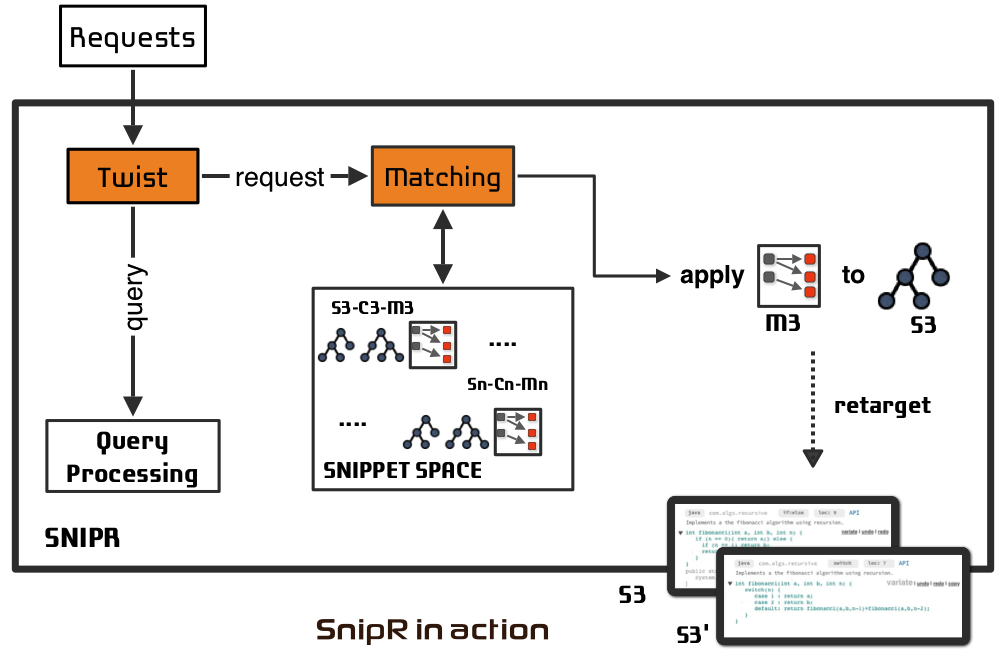
\includegraphics[width=2.8in]{images/halfsnipr}
    \caption{\uppercase{SnipR}'s conceptual architecture. Twist is SNIPR's command line language. 
    The SNIPPET SPACE is where we store of all the 
    possible snippets-mappings generated by humans; where S3 \& C3 are related snippets, and M3 
    is the mapping between these snippets. Matching represents the matching logic for assigning and applying  
    a code mapping to a user request. S3' represents the modified S3 containing the changes specified 
    by M3.}
    \label{fig:architecture}
\end{figure}

The \uppercase{SnipR} approach will be examined by addressing the following research questions:

\begin{itemize}  
\item[RQ1] What kind of \uppercase{SnipR} operations could be invoked directly from the search box?
\item[RQ2] How are these code retargeting capabilities defined and applied?
\item[RQ3] How computationally expensive is it to retarget (part of) examples each time?
\item[RQ4] How does the time needed to perform a more complete code search task of the SnipR approach compare to the current approaches of code search? 
\end{itemize}

\begin{figure}[!t]
    \centering
    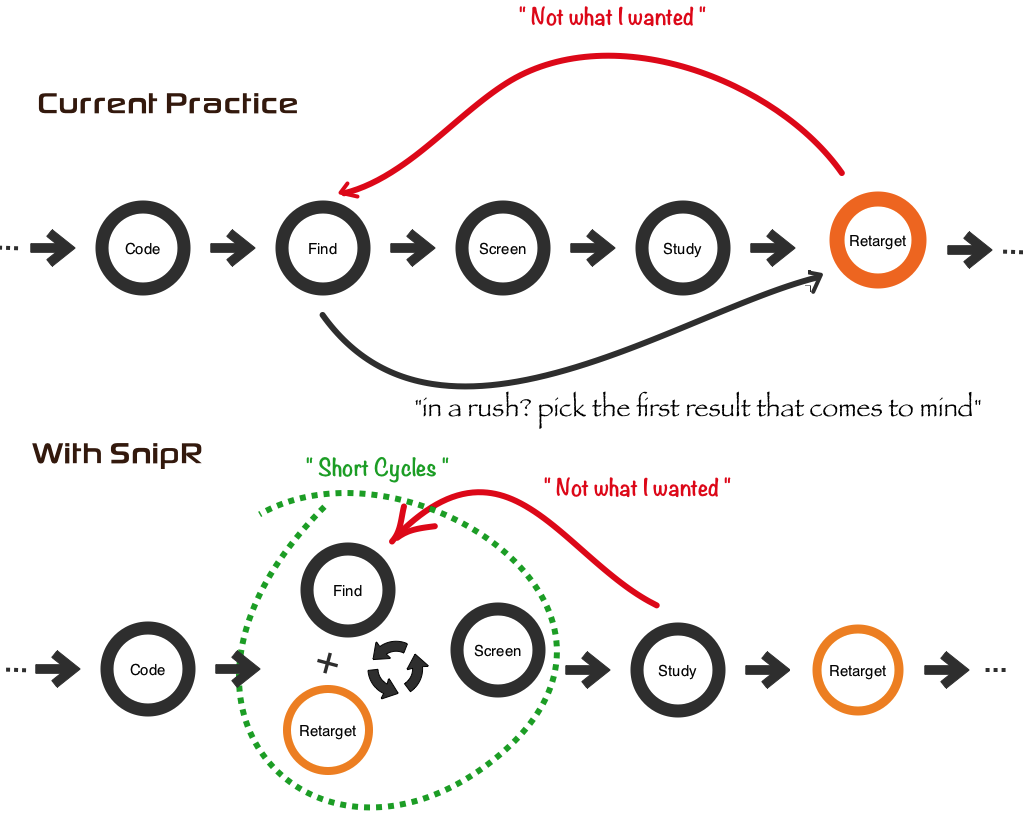
\includegraphics[width=2.8in]{images/halfsearchprocess}
    \caption{Search Process before and with \uppercase{SnipR}. A pre--\uppercase{SnipR} scenario requires developers to find and select the most promising examples (i.e., screening), and then to peruse them before eventually consuming them in the IDE. If the resulting code is not the desired code, then the search process is restarted. With \uppercase{SnipR}, developers engage in a virtuous loop where they find and select only choices they can justify as suitable.}
    \label{fig:retargeting}
\end{figure}
For RQ1, Twist, a command line language for search results interaction and code retargeting is proposed. Twist allows requests for results (queries) and retargeting operations (commands) to be intermixed or used separately. With Twist, developers can not only search for code, but also combine code formatting with removal of redundant code and applying general coding conventions (e.g., reorder type members), all directly from the search box. Figure~\ref{fig:twistcmd} gives an example of Twist's expression. For RQ2, a small Web-based application will be proposed. This application will encourage developers to create code mappings by copying, pasting, and translating prompted code examples to the structure of other examples. These mappings will be saved in SNIPR's SNIPPET SPACE (see Figure~\ref{fig:architecture}). The expected workflow between the developer and this small Web app is illustrated in Figure~\ref{fig:workflow}. 

\begin{figure}[!t]
    \centering
    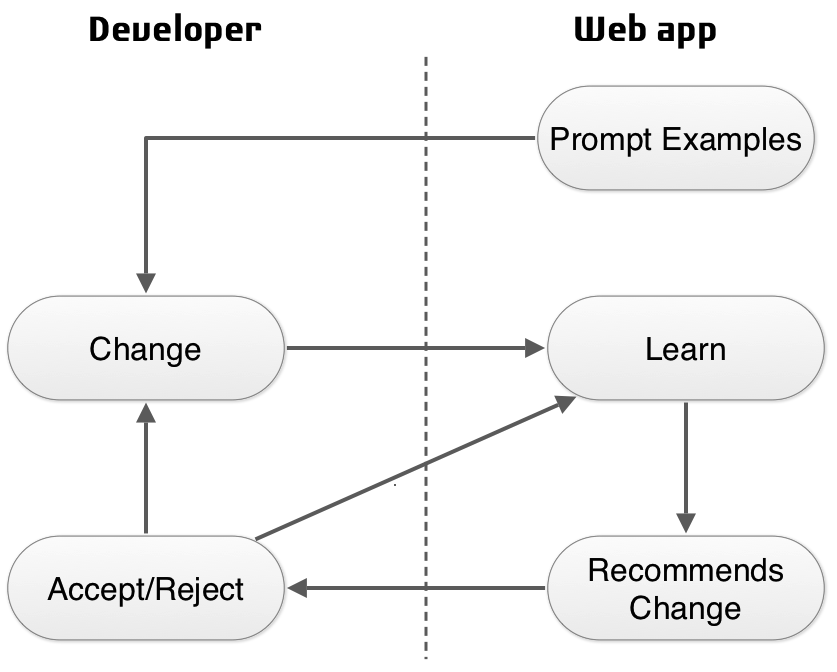
\includegraphics[width=2.8in]{images/workflow}
    \caption{The expected workflow between the developer and the Web app.}
    \label{fig:workflow}
\end{figure}

\begin{figure}[!t]
    \centering
    
\includegraphics[width=2.8in]{images/twistcmd}
    \caption{An expression in Twist: Find all the modules containing the words 
    fibonacci and series, and matching +Int=$>$Array[Int] type signature. Then, 
    reformat each result and then make each result's fields read-only.}
    \label{fig:twistcmd}
\end{figure}

RQ3 is about the performance (in terms of computational throughput) of the code retargeting algorithms. In other words, this is about how long it will take to find the right code mapping and apply it to a particular code snippet. Code retargeting is an operation that can operate on a single result or an entire result set. Therefore, this operation requires that those cases where code mappings can be applied are carefully identified, to prevent any unnecessary work. For RQ4, an evaluation of the efficiency of the \uppercase{SnipR} approach vs. existing approaches for code search is performed. 
 % Of the various sources of information developers find on the Web, example code is the most popular choice since they demonstrate how one should use an given API~\cite{Robillard:2009cs}. Tool support for predetermining whether any ranked example code is a best fit for one’s code is still non-existent. Researchers in search-driven development have tackled 

These solutions are the expected contributions in search-driven development. For the rest of the paper, the focus will shift to the proposed solution to RQ1 (Section~\ref{sec:rq1}), and to a brief description of RQ2, RQ3, and RQ4 in Section~\ref{sec:restqs}. Section~\ref{sec:evaluate} briefly describes a plan for evaluating this work. Section~\ref{sec:progress} outlines the progress to date and Section~\ref{sec:conclude} concludes this paper. 

\section{Proposed Solutions}
\subsection{Designing \uppercase{SnipR} Operations That Could Be Invoked Directly From The Search Box (RQ1)}
\label{sec:rq1}
The key idea is to design a set of retargeting operations that could be invoked from the search box, without losing any sight of the current search goal. This design should balance two inter-related principles: ease of use and flexibility. To understand what's needed to produce this type of design, I'll turn to the seminal work on sloppy command lines for the Web~\cite{Little:2007dh, Miller:2008ge} and on platform-specific linguistic command lines~\cite{Raskin:2008wb}. Similar to both types of work, \uppercase{SnipR}'s Twist will have flexible syntax requirements. This flexibility allows requests for results and retargeting operations to be intermixed---or used separately. The focus of these operations will be on performing code modifications to found examples. Consequently, for ease of use, \uppercase{SnipR} will provide most of the mechanisms for expression and control of changes that can be made to examples---e.g., remove code redundancies, reorder type members, migrate type to other types, reformat code. For flexibility, a simple language for combining, and executing code retargeting commands will be developed. Twist's syntax is influenced by the Io programming language\footnote{\url{http://iolanguage.org/}}.

Previous work in search interfaces for programming exist~\cite{Brandt:2010tp, Bajracharya:2010um, Hummel:eq, Reiss:2009fu}. Undeniably, these types of search interfaces have improved how developers locate code snippets. Large sets of code examples are just one search away. Clearly, this easy access to such an amazing treasure trove code has a value; however, it also has a significant limitation: they are less effective in dynamic and exploratory scenarios; i.e., when developers are working in an unfamiliar domain. In such a scenario the type and number of examples may quickly change as further searchers are performed. Therefore, locating and understanding snippets can easily become overwhelming for any developer. \uppercase{SnipR} differs from these tools by providing a platform with a particular feature set intended to ease this burden: code retargeting operations. 

\subsection{Performing Code Retargeting (RQ2, RQ3, and RQ4)}
\label{sec:restqs}

Code retargeting is an operation that can work on a single search result or an entire result set. Therefore, this operation requires that those cases where code mappings can be applied are carefully identified. This will prevent any unnecessary work from happening as matched code examples are being returned by the query engine. This requirement will be addressed by developing a set of reliable and cache conscious \uppercase{SnipR} algorithms (RQ2). They should be reliable by consistently applying code mappings to found code examples. They should be cache conscious by exploiting recently read example code if this code must be read again in the future. These algorithms represent the modules required to implement SNIPR functionality. See Figure~\ref{fig:architecture} for details.

% The Setup and Learning steps occur at indexing time. Given a set of indexed snippets, the Setup step populates the Snippet Space (cached snippets) by invoking a code clone searching tool. Then it considers all the possible combinations of (original-clone) pairs and saves them into the Snippet Space. Code clones are needed to realize how \uppercase{SnipR}’s learning algorithm operates: they are related implementations and thus similar. They are also syntactically different and are indeed interchangeable. This knowledge is used by the learning algorithm to hypothesize and map together related code elements between snippets. The output of the Setup step is fed into the Learning step. The Learning step then builds mappings for all the (original-clone) pairs in the Snippet Space. To do that, it induces a translation table over the two snippets' similar structures. This table specifies how two code snippets correspond. Once this table is created, the algorithm uses this table to determine structure translation candidates and then uses structured prediction~\cite{Collins:2002uo} to find an optimal code mapping between the two snippets. 

Given a request (See Figure~\ref{fig:architecture}), Twist interprets this input by searching for a mapping that will make sense of this input. At this point, the Matching step maps the retargeting request to its corresponding optimal mapping and then applies this optimal mapping (the one with the highest explanatory power~\cite{Little:2008hr}) to the original snippet. This should happen with minimal or no cost to the developer. Therefore, these operators should be reliable in the sense of efficiently applying defined mappings (RQ3). If the request is a textual query (a list of words), then the request will be forwarded to the query processing step.

In a dynamic and exploratory scenario, developers using \uppercase{SNIPR} will engage in a virtuous loop where they find and select only suitable choices (See Figure~\ref{fig:retargeting}). This results in less time spent on unsuitable, difficult-to-retarget results. This minimizes the number of iterations and thus time in the search process since the developer is only dealing with suitable choices (RQ4). This will be possible only if \uppercase{SnipR}'s retargeting operations are efficient, which will be demonstrated by answering RQ3.

Previous work in adapting code to alternate contexts and/or to new APIs exist. Such work has helped developers with many development tasks, such as adapting example code to new contexts~\cite{Wightman:2012gc} or to new APIs~\cite{Nita:2010en}. This also includes resolving many simple coding errors quickly\footnote{{Quick Fix Scout: \url{https://code.google.com/p/quick-fix-scout/}}, {EUKLAS: \url{http://www.cs.cmu.edu/~euklas}}}, or suggesting ways for correcting compiler and runtime errors~\cite{Hartmann:2010hx}. \uppercase{SnipR} differs from these tools in focus and approach. \uppercase{SnipR} focuses on helping developers justify the suitability of code examples during their search-driven development activities. The other solutions focus on either specifying and applying a class of program transformations, or creating code integration templates which will assist developers in integrating a snippet into their projects. 

\section{Evaluation}
\label{sec:evaluate}

The evaluation methodology to be followed is to validate the \uppercase{SnipR} approach and results through user and lab studies. The tests will be run on \uppercase{SnipR} prototypes in a working code search system. The user studies will involve a list of subjects, solicited from a public mailing list at a college campus. The subjects will be experienced Web users, have some programming experience, and could type reasonably well. The use and test of the \uppercase{SnipR} prototype will be done on the basis of a programming problem to be solved; aiming to answer the research questions listed in Section~\ref{sec:intro}. For instance,

\begin{itemize}  
\item A user study will be performed to test for the flexibility and ease of use of Twist. The test attempts to determine how intuitive this language is for end-users and how easy is for the end-users to translate their ideas into expressions in Twist. The test is also used to determine how this language might be used in daily development activities and to evaluate some of the decisions made on the design of the language's ``intuitively readable commands.'' Each subject will be instructed on using Twist and the instructed to use only the search box to do any of the assigned tasks. Subjects will be asked to solve a programming problem. Once they have completed the assignment, they will be asked to complete survey about their experience with Twist. The data gathered from this test and survey will be used to answer RQ1.
\item Besides creating and executing a set of microbenchmarks, the same user study will be used to provide a feel for the speed and accuracy of the  \uppercase{SnipR} algorithms. Inputs from the user study will be used to derive an average processing time---in terms of applying code mappings from/to code examples. It is expected that the processing time varies for input sizes of different lengths. From this, one could guess that the average-case running time is polynomial, but that is reasonable for relatively small source code (e.g., less than 40 lines of code~\cite{Brandt:2009ew}), such is the case of example code (RQ3).
\item To evaluate the effectiveness of the small Web app, we will experiment with it in a few cases. For example, we will use it to define the mappings between a set of small programs; one using the Guice dependency injection API, and another using the Spring dependency injection API. Some of the questions we will be asking include: Were we able to express all the mappings in these programs? Were we able to apply them without requiring manual modifications to the original program's source code? Is the approach to defining mappings easy to use? The answers to these questions will allow us to answer RQ2.
% \item To evaluate the effectiveness of the learning algorithm, a hold-out test will be run. A set of mappings extracted from a collected corpus will be used as training data, and another different set of mappings---randomly chosen---as a test data. Then a machine learning algorithm will be run for a given number of iterations. The output of this will be a set of mapping-based program transformations. Then, we will use different metrics---e.g., average similarity---to compare the learned and reference mappings. 
\item Another user study will be conducted comparing \uppercase{SnipR} to a general Web code search engine (e.g., Ohloh code) and an example-centric programming tool (e.g., Blueprint). This study attempts to examine how quickly developers perform a more complete code search task (with or without \uppercase{SnipR}). Subjects will be asked to solve a programming problem. Subjects are instructed not to write any code from scratch, but instead to use these tools to find code examples. The order in which search interfaces are presented is controlled by a Latin Square design. The data gathered from this study will be used to answer RQ4.       
\end{itemize}

\section{Progress to Date}
\label{sec:progress}
This work is still at early stages. Work in progress includes my advancement to candidacy by the end of next month, and an early design of the command line language for retargeting source code. The development of code retargeting algorithms, the realization of the \uppercase{SnipR} conceptual architecture, and the implementation of SNIPR's Twist language are work that remains.

\section{Conclusion}
\label{sec:conclude}
This paper has introduced \uppercase{SnipR}, a search application that complements code search with code retargeting capabilities. Unlike prior work, the \uppercase{SnipR} enables developers to engage in a virtuous loop where they find and select only the code examples they can justify as suitable. This will minimize the number of iterations in the search process that developer has to go through, since the evaluation step is only dealing with suitable choices. It is envisioned that \uppercase{SnipR} will not be seen as a competitor to any code search systems, but more like a platform for searching for suitable code.


% references section

% can use a bibliography generated by BibTeX as a .bbl file
% BibTeX documentation can be easily obtained at:
% http://www.ctan.org/tex-archive/biblio/bibtex/contrib/doc/
% The IEEEtran BibTeX style support page is at:
% http://www.michaelshell.org/tex/ieeetran/bibtex/
\bibliographystyle{IEEEtran}
% argument is your BibTeX string definitions and bibliography database(s)
\bibliography{IEEEabrv,icscdocsym}
%
  
\end{document}
